\documentclass[10pt]{report}
\usepackage[utf8]{inputenc}
\usepackage[dutch]{babel}
\usepackage{multicol}
\usepackage[a4paper, margin=0.98in]{geometry}
\usepackage[fleqn]{amsmath}
\usepackage{amsfonts}
\usepackage{titling}
\usepackage{sectsty}
\usepackage{pgfplots}
\usepackage{pgfplotstable}
\usepackage{multirow}
\usepackage{hyperref}
\usepackage{makecell}
\usepackage{fancyhdr}
\usepackage{minted}

\pgfplotsset{compat=newest}

% Header sizes
\sectionfont{\fontsize{11}{14}\selectfont}
\subsectionfont{\fontsize{10}{13}\selectfont}
\subsubsectionfont{\fontsize{9}{12}\selectfont}

% Plot colors
\definecolor{Earth}{rgb}{0.368417,0.506779,0.709798}
\definecolor{Garnet}{rgb}{0.880722,0.611041,0.142051}
\definecolor{Opal}{rgb}{0.560181,0.691569,0.194885}
\definecolor{Sapphire}{rgb}{0.922526,0.385626,0.209179}
\definecolor{Steel}{rgb}{0.528488,0.470624,0.701351}
\definecolor{Sunrise}{rgb}{0.772079,0.431554,0.102387}

% Header and footers
\pagestyle{fancy}
\fancyhf{}
\rfoot{}

% Title page
\author{Laurens Ketsman}
\title{Automatisering van zuur-base titraties - notities bij bronnen}
\date{\today}

% Section numbering
\setcounter{secnumdepth}{5}

% Graphics path
\graphicspath{{img/}}

% minted code style
\usemintedstyle{vs}

% custom commands
\newcommand{\overbar}[1]{\mkern 1.5mu\overline{\mkern-1.5mu#1\mkern-1.5mu}\mkern 1.5mu}

\begin{document}

\clearpage\maketitle
\thispagestyle{empty}
\newpage

\rhead{Pagina \thepage}
\lhead{Laurens Ketsman - 6TTW - Automatisering van zuur-base titraties}

\subsection{Libretext - Labotechnieken titraties}
\begin{itemize}
    \item url: \url{chem.libretexts.org/Core/Analytical_Chemistry/Lab_Techniques/Titration}
\end{itemize}
\textbf{Titratie basistheorie}
\begin{itemize}
    \item $M_1V_1 = M_2V_2$
    \item standaard oplossing = oplossing met gekende concentratie
    \item equivalentiepunt = het ideale eindpunt van een titratie (aantal mol titrant = aantal mol analyt)
    \item eindpunt = zegt wanneer het equivalentiepunt is bereikt, meestal dmv een indicator
    \item eindpunt != equivalentiepunt, ze stellen niet hetzelfde idee voor, equivalentiepunt = theoretisch, eindpunt = praktisch
    \item \textbf{Types titraties}
        \begin{itemize}
            \item \textbf{zuur-base titraties}
                \begin{itemize}
                    \item sterk zuur + sterke base
                    \item zwak zuur + sterke base
                    \item sterk zuur + zwakke base
                    \item zwak polyprotisch zuur (bv. $H_2CO_3$)
                    \item pH = 7 = equivalentiepunt want zuur-base titratie gaat uit van neutralizatiereactie
                \end{itemize}
            \item \textbf{Redoxtitraties}
                \begin{itemize}
                    \item red $\rightarrow$ reducerend, ox $\rightarrow$ oxygen $\rightarrow$ zuurstof
                    \item doel = bepalen van overdracht van $e^-$ van 1 stof naar de andere.
                    \item eindpunt kan gemeten worden dmv potentiometer of kleurveranderende indicator
                \end{itemize}
            \item \textbf{Combinatie reactie titraties}
                \begin{itemize}
                    \item \textbf{Neerslagtitraties}
                        \begin{itemize}
                            \item titratie van 2 tegengestelde ionen bv $Ag^+$ end $Cl^-$
                            \item vormt niet altijd een neerslag dus indicator is soms nodig
                            \item als er een neerslag word gevormd is dit ook het eindpunt van de titratie
                        \end{itemize}
                    \item \textbf{Complextitraties}
                        \begin{itemize}
                            \item EDTA = ethyleendiaminetetraacetaatzuur
                                \begin{figure}[h]
                                    \centering
                                    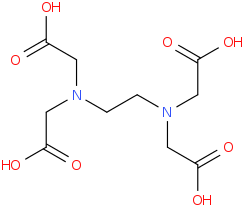
\includegraphics[width=0.2\textwidth]{EDTA.png}
                                    \caption{EDTA}
                                \end{figure}
                            \item word gebruikt voor titratie van metaalionen
                        \end{itemize}
                \end{itemize}
        \end{itemize}
    \item \textbf{Titratiecurves}
        \begin{itemize}
            \item titratiecurves tonen het verband tussen de pH van de te bepalen oplossing en het aantal mol titrant dat is toegevoegd
        \end{itemize}
\end{itemize}
\newpage
\textbf{Zuur base titraties}
\begin{itemize}
    \item zuur base titraties gaan uit van een neutralizatiereactie bv. $HCl_{(aq)} + NaOH_{(aq)} \rightarrow Na^+ + Cl^- + H_2O$
    \item opgelost $CO_2$ kan een rol spelen omdat $CO_2 + H_2O \rightarrow H_2CO_3$ de pH zal beïnvloeden.
\end{itemize}
\textbf{Titratie van sterk zuur met sterke base}
\begin{itemize}
    \item makkelijkste van de 4 want beide dissocieren volledig in water
    \item doel is om de concentratie van een zuur (of base) te bepalen dmv een neutralizatiereactie $\rightarrow$ het equivalentiepunt is dus wanneer pH 7 bereikt is
    \item Sterke zuren en basen\\\\
        \begin{tabular}{|l|l|}
            \hline
            Zuren & Basen \\\hline
            $HCl$ & $LiOH$ \\\hline
            $HBr$ & $NaOH$ \\\hline
            $HI$ & $KOH$ \\\hline
            $HClO_4$ & $RbOH$ \\\hline
            $HNO_3$ & $CsOH$ \\\hline
            $H_2SO_4$ & $Mg(OH)_2$ \\\hline
            & $Ca(OH)_2$ \\\hline
            & $Sr(OH)_2$ \\\hline
            & $Ba(OH)_2$ \\\hline
        \end{tabular}
        \item Veel uitgewerkte voorbeelden in bron
\end{itemize}
\textbf{Titratie van zwak zuur met sterke base}
\begin{itemize}
    \item \textbf{Eigenschappen titratiecurve}
        \begin{itemize}
            \item De initiele pH (voor er een sterke base is aan toegevoegd) is hoger dan de titratie van een sterk zuur
            \item Er is een scherpe stijging van de pH in het begin van de titratie
            \item Na de scherpe stijging stijgt de pH maar matig
            \item In het midden van de matige stijging ligt het halfneutralizatiepunt (waar de afgeleide 0 is), op dit punt is de concentratie van het zwakke zuur gelijk aan de concentratie van de geconjugeerde base (pH=pK\textsubscript{a}). Dit noemt het halfneutralizatiepunt omdat op dat punt de helft van het zuur geneutralizeerd is
            \item Op het equivalentiepunt is de pH groter van 7 omdat al het zuur omgezet is in de geconjugeerde base
            \item The sterk stijgend stuk van de titratiecurve is kort en gebeurd meestal maar rond een pH van 10
        \end{itemize}
    \item Veel uitgewerkte voorbeelden in bron
\end{itemize}
\textbf{Titratie van zwakke base met sterk zuur}
\begin{itemize}
    \item Halfneutralizatiepunt is waar de titratiecurve vlak is (afgeleide is 0)
\end{itemize}
\textbf{Titratie van een zwak polyprotisch zuur} 
\begin{itemize}
    \item een zwak polyprotisch zuur is een zuur die meerdere protonen ($H^+$ ionen) kan doneren en niet volledig dissocieerd in water. bv. $H_3PO_4$, $H_2CO_3$
    \newpage
    \begin{figure}[h]
        \centering
        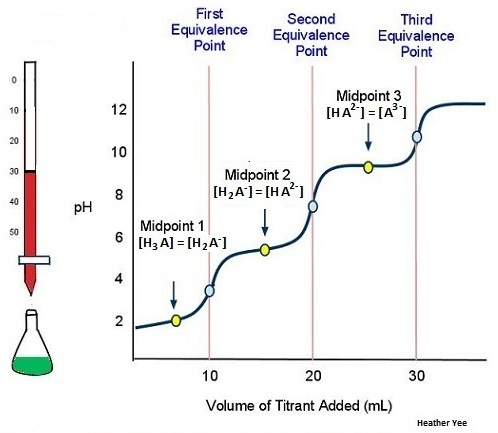
\includegraphics[width=0.6\textwidth]{TitratieZwakMeervoudigZuur.jpg}
        \caption{Titratie van een zwak polyprotisch zuur. Afbeelding gemaakt door Heather Yee.}
    \end{figure}
    \item \textbf{Eigenschappen titratiecurve}
        \begin{itemize}
            \item De curve start op een hogere pH dan een titratie van een sterke base
            \item Er is een sterke stijging voor het eerste middenpunt (afgeleide = 0)
            \item Matige stijging na het eerste middenpunt
            \item Vlak voor het eerste equivalentiepunt is er een sterke stijging
            \item De pH stabiliseerd zich dan rond het volgende middenpunt
            \item Bovenstaande eigenschappen worden herhaald
        \end{itemize}
    \item Veel uitgewerkte voorbeelden in bron
\end{itemize}

\subsection{Chemguide - pH curves}
\begin{itemize}
    \item url: \url{chemguide.co.uk/physical/acidbaseeqia/phcurves.html}
\end{itemize}
\textbf{Termen}
\begin{itemize}
    \item Neutraal punt: punt waar de oplossing pH 7 heeft
    \item equivalentiepunt: punt waar de 2 oplossingen met exact de juiste verhouding met elkaar gemengd zijn
    \item eindpunt: punt waar de indicator het einde van de titratie aangeeft
\end{itemize}
\newpage
\textbf{Titratiecurves}
\begin{itemize}
    \item \textbf{Sterk zuur + sterke base}
        \begin{figure}[h]
            \centering
            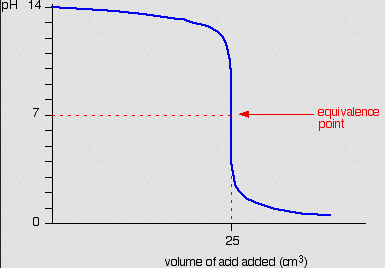
\includegraphics[width=0.4\textwidth]{SterkZuurSterkeBaseCurve.png}
            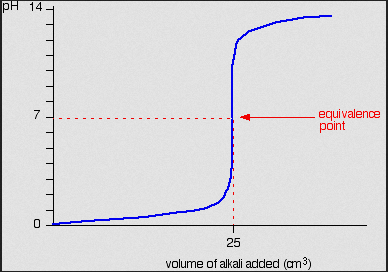
\includegraphics[width=0.4\textwidth]{SterkZuurSterkeBaseCurve2.png}
            \caption{Titratiecurve van een sterk zuur met een sterke base}
        \end{figure}
    \item \textbf{Sterk zuur + zwakke base}
        \begin{figure}[h]
            \centering
            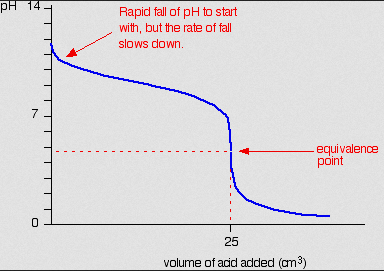
\includegraphics[width=0.4\textwidth]{SterkZuurZwakkeBaseCurve.png}
            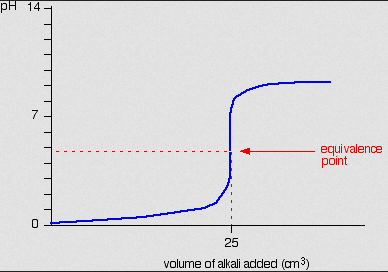
\includegraphics[width=0.4\textwidth]{SterkZuurZwakkeBaseCurve2.png}
            \caption{Titratiecurve van een sterk zuur met een zwakke base}
        \end{figure}
    \item \textbf{Zwak zuur + sterke base}
        \begin{figure}[h]
            \centering
            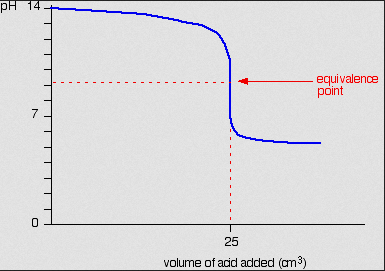
\includegraphics[width=0.4\textwidth]{ZwakZuurSterkeBaseCurve.png}
            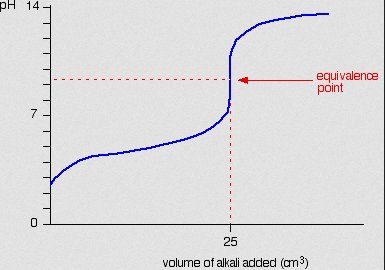
\includegraphics[width=0.4\textwidth]{ZwakZuurSterkeBaseCurve2.png}
            \caption{Titratiecurve van een zwak zuur met een sterke base}
        \end{figure}
    \newpage
    \item \textbf{Zwak zuur + zwakke base}
        \begin{figure}[h]
            \centering
            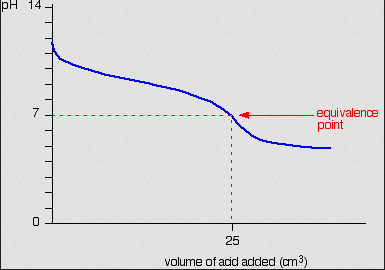
\includegraphics[width=0.4\textwidth]{ZwakZuurZwakkeBaseCurve.png}
            \caption{Titratiecurve van een zwak zuur met een zwakke base}
        \end{figure}
\end{itemize}

\subsection{Zomercursus chemie KUL - zuur-base reacties}
\begin{itemize}
    \item
        \begin{equation*}
            \begin{split}
                pH + pOH &= 14 \\
                pOH &= -log([OH^-]) \\
                [H_3O^+][OH^-] &= 10^{-14} \\
                k_a &= \frac{[A^-]_e.[H_3O^+]_e}{[HA]_e} \\
                k_b &= \frac{[HA]_e.[OH^-]_e}{[A^-]_e} \\
                k_ak_b &= \frac{[A^-]_e[H_3O^+]_e[HA]_e[OH^-]_e}{[HA]_e[A^-]_e} = [H_3O^+]_e[OH^-]_e
            \end{split}
        \end{equation*}
    \item polyprotisch zuur = een zuur die meer dan 1 afsplitsbaar proton bevat
    \item bij polyprotische zuren komen er 2 evenwichten tot stand en dus ook 2 zuurconstanten
    \item bv. $H_2SO_4$
        \begin{equation*}
            \begin{split}
                H_2SO_4 + H_2O &\rightarrow HSO_4^- + H_3O^+ &, k_{a_1} &= \frac{[HSO_4^-][H_3O^+]}{[H_2SO_4]} \\
                HSO_4^- + H_2O &\rightleftharpoons SO_4^{2-} + H_3O^+ &, k_{a_2} &= \frac{[SO_4^{2-}][H_3O^+]}{[HSO_4^-}
            \end{split}
        \end{equation*}
    \item de 2\textsuperscript{de} zuurconstante is dus altijd kleiner dan de eerste enz.
\end{itemize}

\subsection{mcat-review - acids-bases}
\begin{itemize}
    \item url: \url{mcat-review.org/acids-bases.php}
\end{itemize}
\begin{equation*}
    \begin{split}
        HA &+ B^- &\rightarrow A^- &+ HB
    \end{split}
\end{equation*}
\begin{itemize}
    \item van links naar rechts:
        \begin{itemize}
            \item Zuur: proton donor
            \item Base: proton acceptor
            \item Geconjugeerde base: zuur na verlies van proton
            \item Geconjugeerde zuur: base met proton
        \end{itemize}
    \item $k_w = [H^+][OH^-] = 10^{-14}$ bij $25^\circ C$
    \item $H_2O \rightleftharpoons H^+ + OH^-$
\end{itemize}
\begin{figure}
    \centering
    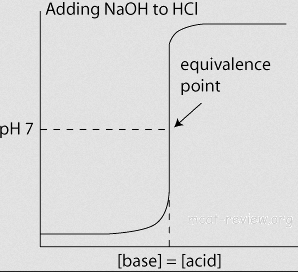
\includegraphics[width=0.3\textwidth]{mcat0.png}
    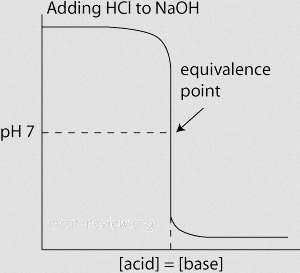
\includegraphics[width=0.3\textwidth]{mcat1.png}
    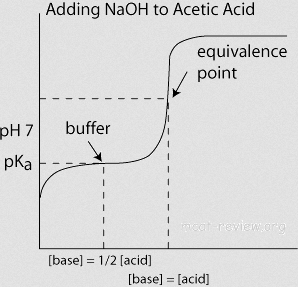
\includegraphics[width=0.3\textwidth]{mcat2.png}
    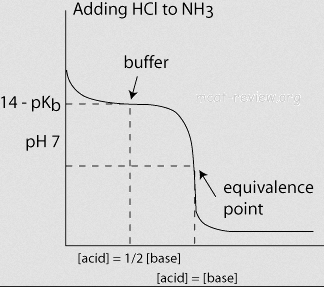
\includegraphics[width=0.3\textwidth]{mcat3.png}
    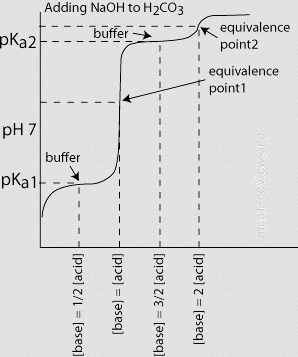
\includegraphics[width=0.3\textwidth]{mcat4.png}
\end{figure}

\subsection{rfpc.ir - Basics of titration}
\begin{itemize}
    \item url: \url{http://www.rfpc.ir/uploads/Basics_of_Titration.pdf}
\end{itemize}
\begin{itemize}
    \item Titratie = een analytische techniek die toelaat om de concentratie van een stof te bepalen in oplossing
    \item bv. $CH_3COOH + NaOH \rightarrow CH_3COO^- + Na^+ + H_2O$
    \item De reactie bij een titratie moet snel, compleet, ondubbelzinnig en observeerbaar zijn
    \item \textbf{Geschiedenis}
        \begin{itemize}
            \item Vroeger:
            \begin{itemize}
                \item titratie is een klassieke en veelgebruikte techniek.
                \item buret + kleurindicator
                \item precisie hing vooral af van de bekwaamheid van de chemicus
            \end{itemize}
            \item Nu:
            \begin{itemize}
                \item automatisch via elektronisch aangedreven buretten, sensoren en microcontrollers
            \end{itemize}
        \end{itemize}
    \item \textbf{Titratie theorie}
        \begin{itemize}
            \item zuur-base reacties zoals $HCl + NaOH \rightarrow NaCl + H_2O$, voorbeelden: zuurgehalte wijn ($HCl$), melk ($HNO_3$), ketchup ($H_2SO_4$)
            \item EQP = equivalence point = equivalentiepunt
            \item in meeste gevallen EQP = inflectiepunt grafiek ($E (mV)$ in functie van $V (mL)$
            \item titratie komt voor in volgende werkvelden: Landbouw, luchtvaart, bouwmaterialen, productie van wagens, chemische industrie, kool producten, coatings, cosmetische producten, detergenten, drugs, elektronische industrie, energie, explosieven, voedsel, glass, overheid, gezondheid, leder, machines, pharmacie, leger, ontginning, olie-industrie, verpakking, verven en pigmenten, papier en pulp, petroleum, foto industrie, platiscs, drukwerk, rubber, zeep, treinen, steen, textiel, universiteiten en scholen, water, mineralen etc
            \newpage
            \item voordelen van titratie:
                \begin{itemize}
                    \item welgekende techniek
                    \item snel
                    \item zeer precies
                    \item kan geautomatiseerd worden
                    \item goede prijs/kwaliteit
                    \item kan gedaan worden door zonder veel scholing
                    \item geen nood voor zeer gespecializeerde chemische kennis
                \end{itemize}
        \end{itemize}
    \item \textbf{Automatische titratie}
        \begin{itemize}
            \item Automatische titrator = een instrument die toelaat de toevoeging van titrant, observeren van reactie, herkenning van het eindpunt, opslag van gegevens, berekening van resultaten en opslag te automatiseren
            \begin{figure}[h]
                \centering
                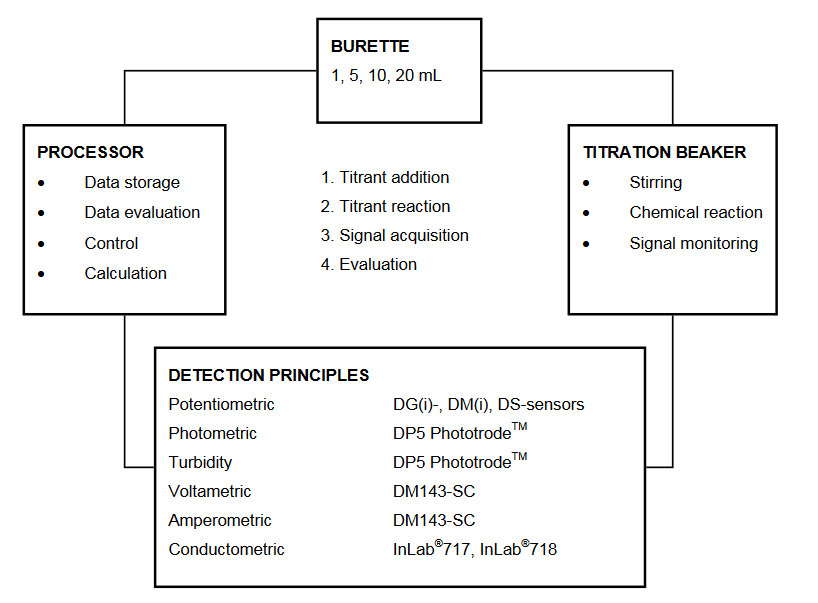
\includegraphics[width=1\textwidth]{rfpcir.png}
                \caption{Schematische voorstelling van verschillende stappen in een automatische titratie}
            \end{figure}
            \item \textbf{Toevoeging van titrant}
                \begin{itemize}
                    \item incrementele titrant toevoeging
                        \begin{itemize}
                            \item titrant word toegevoegd in constante volumes $\Delta V$ \newpage
                                \begin{figure}[h]
                                    \centering
                                    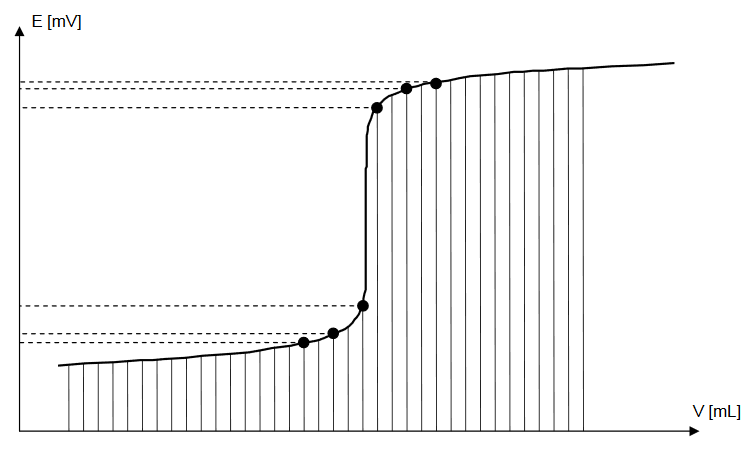
\includegraphics[width=0.7\textwidth]{rfpcir2.png}
                                    \caption{Incrementele toevoeging van titrant}
                                \end{figure}
                        \end{itemize}
                    \item dynamische titrant toevoeging
                        \begin{itemize}
                            \item $\Delta V$ is veranderlijk en gebaseerd op voorgedefinieerde parameters en de titratiecurve
                                \begin{figure}[h]
                                    \centering
                                    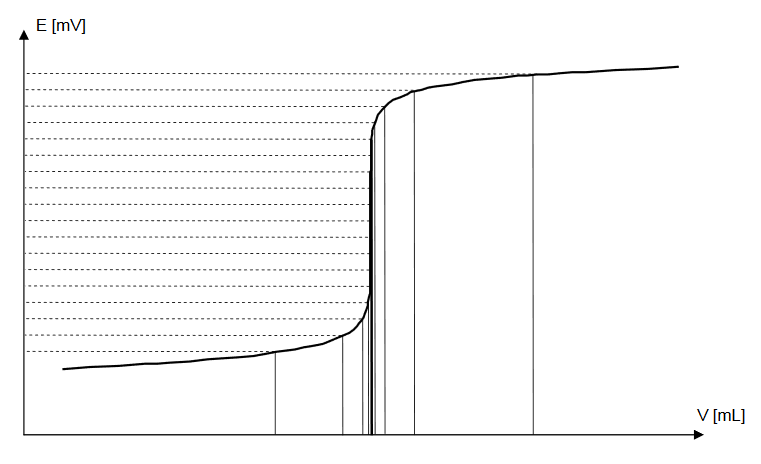
\includegraphics[width=0.7\textwidth]{rfpcir3.png}
                                    \caption{Dynamische toevoeging van titrant}
                                \end{figure}
                        \end{itemize}
                    \item lopende titrant toevoeging
                        \begin{itemize}
                            \item titrant word toegevoegd in een constant tempo tot een zeker punt is bereikt, word vooral gebruikt in eindpuntitraties
                        \end{itemize}
                \end{itemize}
            \newpage
            \item Meten van waarden
                \begin{itemize}
                    \item Tijdsgebaseerde verzameling
                        \begin{figure}[h]
                            \centering
                            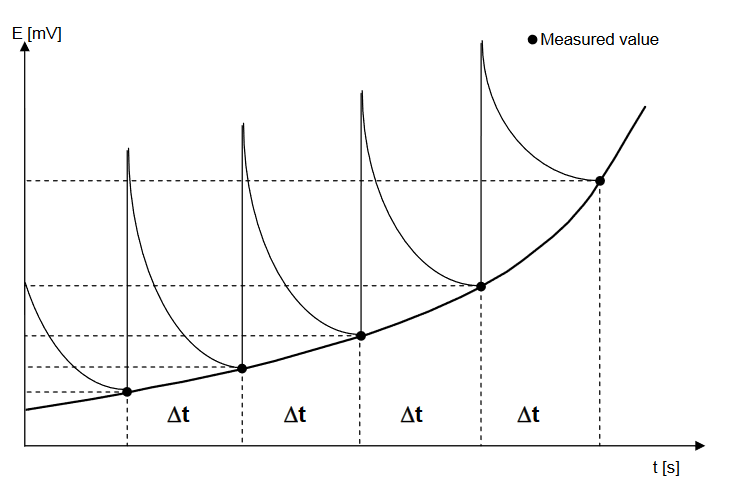
\includegraphics[width=0.7\textwidth]{rfpcir4.png}
                            \caption{Tijdsgebaseerde verzameling van data}
                        \end{figure}
                    \item Evenwichtsgecontroleerde verzameling
                        \begin{figure}[h]
                            \centering
                            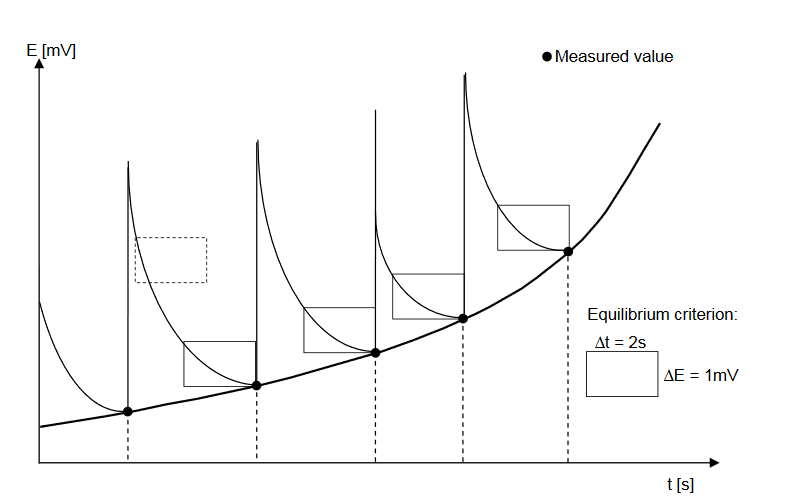
\includegraphics[width=0.7\textwidth]{rfpcir5.png}
                            \caption{Evenwichtsgecontroleerde verzameling van data}
                        \end{figure}
                \end{itemize}
            \newpage
            \item Evaluatie principes
                \begin{itemize}
                    \item Symmetrische S-vormige curve
                        \begin{figure}[h]
                            \centering
                            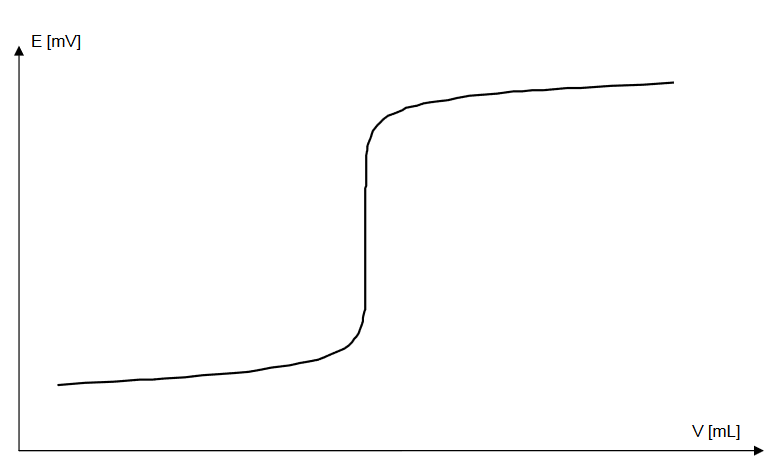
\includegraphics[width=0.7\textwidth]{rfpcir6.png}
                            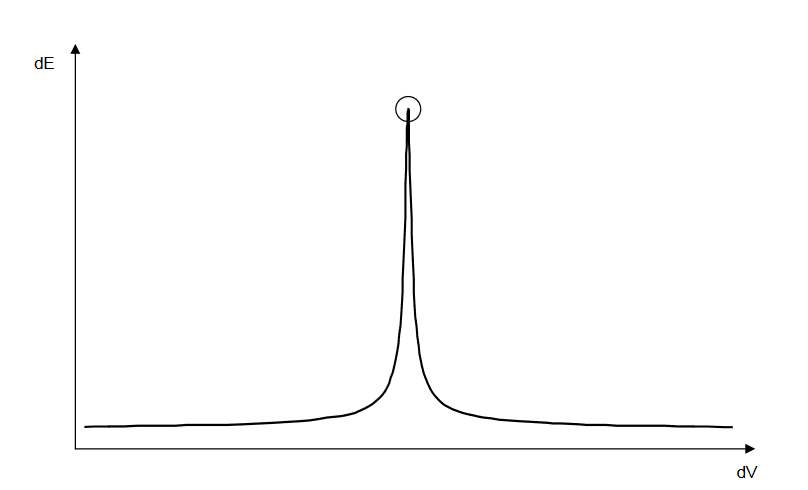
\includegraphics[width=0.7\textwidth]{rfpcir7.png}
                            \caption{Symmetrische S-vormige titratiecurve en de eerste afgeleide ervan}
                        \end{figure}
                        \begin{itemize}
                            \item Het maximum van de eerste afgeleide vertaald naar het EQP van de curve
                        \end{itemize}
                    \newpage
                    \item Asymmetrische curve
                        \begin{figure}[h]
                            \centering
                            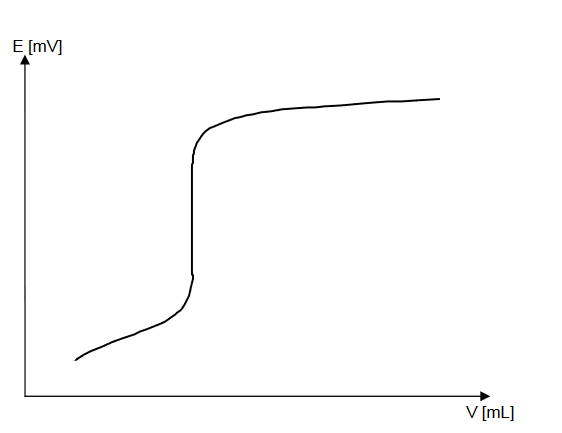
\includegraphics[width=0.7\textwidth]{rfpcir8.png}
                            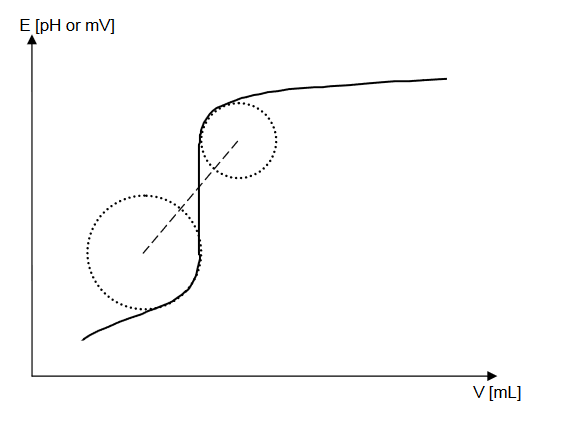
\includegraphics[width=0.7\textwidth]{rfpcir9.png}
                            \caption{Asymmetrische curve en analyze}
                        \end{figure}
                        \begin{itemize}
                            \item De curve word gefit met 2 cirkels, de snijding van de lijn die loopt van het 1ne middelpunt naar het andere met de curve is het EQP
                        \end{itemize}
                \end{itemize}
            \newpage
            \item Nauwkeurigheid, precisie en juistheid
                \begin{itemize}
                    \item juistheid: hoe dicht het gemiddelde van alle metingen bij de echte waarde ligt 
                        \begin{equation*}
                            b = \frac{\sum{x_i}}{n} - r
                        \end{equation*}
                    \item precisie: hoe dicht waarden bij elkaar liggen in een individuele serie van metingen, word gegeven door de standaardafwijking of de relatieve standaard afwijking van een serie van metingen
                        \begin{equation*}
                            \begin{split}
                                s &= \sqrt{\frac{1}{n-1}\sum_{i=1}^n{(x_i - \frac{\sum{x_i}}{n})^2}}\\
                                srel &= \frac{s}{\frac{\sum{x_i}}{n}}.100
                            \end{split}
                        \end{equation*}
                    \item nauwkeurigheid is de combinatie precisie en juistheid
                \end{itemize}
            \item Fouten:
                \begin{itemize}
                    \item Systematische fouten:
                        \begin{itemize}
                            \item Verschillende of foute analytische methode
                            \item Foute formules
                            \item Monster fouten
                            \item Monstergrote fouten
                            \item Foute concentratie van titrant
                            \item Foute of afwezige waarden
                            \item Foute sensor regeling
                            \item Te hoge titratiesnelheid voor gegeven reactie
                        \end{itemize}
                    \item Willekeurige fouten
                        \begin{itemize}
                            \item Fout hanteren van monsters
                            \item Onvoldoende precies materiaal
                            \item Foute parameters
                            \item Luchtbellen in buret
                            \item Onvoldoende reiniging
                            \item Onvoldoende training van operator
                            \item Temperatuurs en vochttigheidsfluctuaties
                        \end{itemize}
                    \item grove fouten
                        \begin{itemize}
                            \item Notitiefouten
                            \item Berekeningsfouten
                        \end{itemize}
                \end{itemize}
            \item Juiste parameters kiezen
                \begin{figure}[h]
                    \centering
                    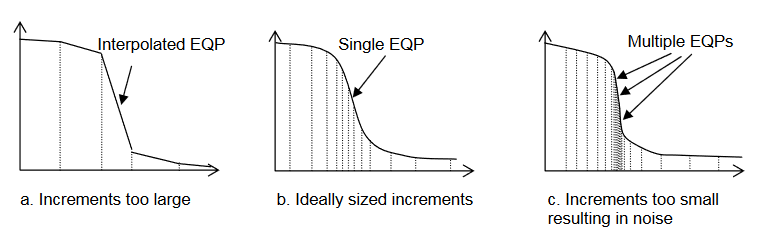
\includegraphics[width=1\textwidth]{rfpcir10.png}
                    \caption{Increment grootte en dynamische toevoeging van titrant}
                \end{figure}
        \end{itemize}
    \item Achtergrond chemie
        \begin{itemize}
            \item $1$ mol = $6.025E^{23}$ deeltjes
            \begin{equation*}
                aA + bB \rightleftharpoons xX + yY
            \end{equation*}
            \item a,b,x,y zijn het aantal er aanwezig is van A,B,X,Y, evenwicht is bereikt wanneer de snelheid van de heengaande reactie gelijk is aan de snelheid van de teruggaande reactie, $v_1 = v_2$
            \begin{equation*}
                K = \frac{[X]^x[Y]^y}{[A]^a[B]^b}
            \end{equation*}
            \item $K$ is de evenwichtsconstante
            \begin{equation*}
                K_{sp} = \frac{[A^+][B^-]}{[AB]}
            \end{equation*}
            \item $K_{sp}$ is hier het oplossingsproduct
            \begin{equation*}
                \begin{split}
                    2H_2O &\rightleftharpoons H_3O^+ + OH^-\\
                    K_w &= [H_3O^+][OH^-]\\
                    [H_3O^+] &= [OH^-] = 10^{-7} mol/L
                \end{split}
            \end{equation*}
            \item ionisatie van water
            \begin{equation*}
                \begin{split}
                    HA &+ H_2O \rightleftharpoons H_3O^+ + A^-\\
                    K_a &= \frac{[H_3O^+][A^-]}{[HA]}
                \end{split}
            \end{equation*}
            \item $K_a$ is de zuurconstante
            \begin{equation*}
                pK_a = -log(K_a)
            \end{equation*}    
        \end{itemize}
\end{itemize}

\subsection{Instructables - Arduino based chemical titration}
\begin{itemize}
    \item url: \url{instructables.com/id/Arduino-Based-Chemical-Titration-aka-The-Titration}
\end{itemize}
\begin{itemize}
    \item Arduino circuit terugtevinden in bron
    \item gebruikgemaakt van lichsensor in combinatie met indicator in oplossing
    \item Gebruikte pomp: \url{www.amazon.com/gp/product/B00HIX2PEG/ref=ox_sc_act_title_1?ie=UTF8&psc=1&smid=A388EF2JRGUUQ3}
    \item pomp werd aangestuurd door arduino dmv PWM
\end{itemize}

\subsection{Arduino projects book \& Arduino.cc}
\begin{itemize}
    \item url: \url{arduino.cc/en/Reference/HomePage}
\end{itemize}
\begin{itemize}
    \item Arduino programmeren:
        \begin{itemize}
            \item De basisstructuur van een Arduino programma
        \end{itemize}
\end{itemize}
\begin{minted}
[
linenos
]
{csharp}
// Constructor/initializator, word eenmaal opgevoert wanneer de Arduino opstart
void setup()
{
}

// instructieloop, word uitegevoert na setup() en word constant herhaald
void loop()
{
}
\end{minted}
\begin{itemize}
    \begin{itemize}
        \item Controle structuren: if else, while, do while, for, break, continue, switch, return
    \end{itemize}
\end{itemize}
\begin{minted}
[
linenos
]
{csharp}
if (a < b)
{
// code voor wanneer a kleiner is dan b
}
else
{
// code voor wanneer a niet kleiner is dan b
}

while (a < b)
{
// zolang a kleiner is dan b voor dit uit, word minimaal 0 keer uitgevoerd
}

do
{
// voor deze code uit en evalueer dan a < b, blijft dit herhalen tot wanneer a niet
// meer kleiner is dan b, word minimaal 1 maal uitgevoerd
} while (a < b)

for (int i = 0; i < a; i++)
{
// 1. maak een nieuwe variable i aan met waarde nul
// 2. evalueer dan de expressie i < a
// 3. Voor dan deze code uit als i < a waar is
// 4. Voor dan i++ uit en herhaal vanaf stap 2
}

switch (a)
{
    case b:
        // a == b
        break;
    case c:
        // a == c
        break;
    case d:
        // a == d
        break;
    ...
    default:
        // a != b, a != c, a != d, typeof(a) != typeof(b,c,d)
}

break;    // spring uit een loop
continue; // ga direct naar de volgende iteratie van een loop
return x; // geef x als resultaat van de functie, return; geeft een NULL waarde terug
          // wanneer de functie geen return type heeft
\end{minted}
\begin{itemize}
    \begin{itemize}
        \item Operatoren en samengestelde operatoren
    \end{itemize}
\end{itemize}
\begin{minted}
[
linenos
]
{csharp}
a = b          // geef waarde b aan a
+,-,*,/,\%     // optellen aftrekken, vermenigvuldigen, delen, modulo
a == b, a != b // is a gelijk aan b, is a niet gelijk aan b, geeft een boolean
               // als resultaat
<,>, <=, >=    // kleiner dan, groter dan, kleiner dan of gelijk aan, groter
               // dan of gelijk aan
&&, ||, !      // and, or, not
++, --         // increment en decrement
a += b         // tel b bij a op en steek die waarde terug in a
-=, *=, /=     // samengesteld aftrekken, vermenigvuldigen en delen
&=, |=         // samengestelde bitsgewijze and en or
&, |, ^, ~     // bitsgewijze and, or, xor, not
<<, >>         // linkse en rechtse bitshift
\end{minted}
\begin{itemize}
    \begin{itemize}
        \item Variabelen, arrays en data
    \end{itemize}
\end{itemize}
\begin{minted}
[
linenos
]
{csharp}
// Data types
void            //
boolean         // true, false, 0, 1
char            // 'a', -128 tot 127
int             // -32768 tot 32767
long            // -2147483648 tot 2147483647
unsigned char   // 0 tot 255
byte            // 0 tot 255
unsigned int    // 0 tot 65535
word            // 0 tot 65535
unsigned long   // 0 tot 4294967295
float           // kommagetal
double          // float

// Qualifiers
static   // blijft bestaan tussen calls
volatile // in RAM geheugen
const    // alleen lezen variable
PROGMEM  // in flash

// Pointers
&   // pointer referentie
*   // pointer dereferentie

// Arrays en lijsten
int Ints[2];        // array van 2 variablen van het type int, nog niet
                    // geinitializeerd, strings NULL!
int Ints[] = {a, b};
int Ints[3] = {a};
int Ints[a] = b;    // geef waarde aan de variable met index a in de array
                    // indexen beginnen vanaf 0!

// Tekst
char str[2] = {'a', '\0'}; // strings hebben een NULL terminatie nodig
char str[] = "a";          // automatische NULL terminatie
\end{minted}
\begin{itemize}
    \begin{itemize}
        \item Ingebouwde functies
    \end{itemize}
\end{itemize}
\begin{minted}
[
linenos
]
{csharp}
// Pins
pinMode(pin, INPUT|OUTPUT)  // configureert een pin als input of output
digitalRead(pin)            // leest een waarde van een specifieke digitale pin
digitalWrite(pin, a)        // schrijf HIGH of LOW waarde naar een digitale pin
analogRead(pin)             // leest een waarde van een analoge pin
analogReference(DEFAULT|INTERNAL|EXTERNAL) // configureert het referentie voltage voor een
                                           // analoge input
analogWrite(pin, a) // PWM (pulse with modulation) pins: 3,5,6,9,10,11, a = duty cycle
tone(pin, freqhz)           // genereert een golf met gekozen freq
tone(pin, freqhz, ms)       // ms = duratie van golf
noTone(pin)                 // stopt een golf op een pin
shiftOut(datapin, clockpin, MSBFIRST|LSBFIRST, a) // shifts een byte bit per bit
                            // datapin = output, clockpin = pin die moet aan/af gezet
                            // worden, MSB = most sig bit, LSB = least sig bit
                            // a = data
pulseIn(pin, HIGH|LOW)      // leest lengte van een pulse op een pin

// Tijd
millis()                // aantal ms sinds boot
micros()                // aantal us sinds boot
delay(ms)               // block thread voor ms aantal ms
delayMiroseconds(us)    // block thread voor us aantal us

// Wiskunde
min(a, b)   // minimum
max(a, b)   // maximum
abs(a)      // absolute waarde
sin(rad)    // sinus
cos(rad)    // cosinus
tan(rad)    // tangens
constrain(a, min, max) // beperk een waarde tot bepaald interval
map(a, fl, fh, tl, th) // waarde omzetten tussen intervallen (mappings)
randomSeed(a)          // initializeer de pseudo-random number generator met
                       // gegeven seed (millis()/ micros())
random(max)            // willekeurig getal beperkt tot max
random(min, max)       // willekeurig getal uit interval
lowByte(a)             // leest meest rechtse byte van een variable
highByte(a)            // leest meest linkse byte van een variable
bitRead(a, n)          // leest nde bit van een variable
bitWrite(a, n, b)      // schrijft bit b op plaats n in a
bitSet(a, n)           // bitwrite maar b = 1
bitClear(a, n)         // bitwrite maar b = 0
bit(n)                 // 2^n

// Type omzettingen
char(a)  // variable naar het type char omzetten
byte(a)  // variable naar het type byte omzetten
int(a)   // variable naar het type int omzetten
word(a)  // variable naar het type word omzetten
long(a)  // variable naar het type long omzetten
float(a) // variable naar het type float omzetten

// Interrupts
attachInterrupt(interp, f, LOW|CHANGE|RISING|FALLING)
        // interp = digitalPinToInterrupt(pin), f = interruptfunctie (blink)
        // LOW = trigger wanneer pin in LOW staat is etc
detachInterrupt(interp) // stop interrupt, interp = interrupt nummer
interrupts()
noInterrupts()
\end{minted}
\begin{itemize}
    \begin{itemize}
        \item Externe functies
    \end{itemize}
\end{itemize}
\begin{minted}
[
linenos
]
{csharp}
// Seriële communicatie
begin(spd)      // begin seriële communicatie met gegeven snelheid
end()           // beëindig seriële communicatie
available()     // is seriële communicatie beschikbaar
read()          // lees een byte
peek()          // lees een byte maar verwijder het niet uit de cache 
flush()         // flush de writing cache naar de seriële stream
print(d)        // schrijf d naar writing cache
println(d)      // schrijf d + '\\0' naar writing cache
write()         // schrijf binaire data naar seriele poort
serialEvent()   // word aangeroepen wanneer er data beschikbaar is

// Servo
// servo header niet als referentie vergeten
// #include <Servo.h>
attach(pin)     // start de library op een pin
write(deg)      // zet servo in deg graden stand
read()          // lees stand servo
attached()      // is verbonden met pin?
detach()        // koppeld library los
\end{minted}

\subsection{msdn - system.io.ports.serialport}
\begin{itemize}
    \item url: \url{msdn.microsoft.com/en-us/library/system.io.ports.serialport(v=vs.110).aspx}
\end{itemize}
\begin{itemize}
    \item communicatie met arduino is mogelijk via de seriële poort waarmee het verbonden is met de pc via de system.io.ports.serialport klasse van het .NET framework
    \item compatibiliteit met .NET framework 2 en hoger
    \item public static members van de klasse zijn thread-safe, instance members mogelijks niet
    \item uitgewerkt voorbeeld terugtevinden van hoe de klasse moet gebruikt worden
\end{itemize}
\subsection{Eigen notities}
    \begin{itemize}
        \item Verbinden met Arduino vanuit C\# via seriele poort
    \end{itemize}
\begin{minted}
[
linenos
]
{csharp}
using System;
using System.IO.Ports;

namespace ConnectionTest
{
    public static class Program
    {
        private static void Main(string[] args)
        {
            SerialPort port = new SerialPort("COM3", 9600);
            port.Open();
            while (port.IsOpen)
            {
                Console.WriteLine(port.ReadLine());
            }
        }
    }
}
\end{minted}
\end{document}